% !TeX spellcheck = da_DK
\chapter{Nervefysiologi}\label{AppNerve}
Kroppens nervesysten kan inddeles i to dele; det centrale nervesystem (CNS) og det perifere nervesystem (PNS). CNS inderholder hjernen og rygraden, mens PNS indebærer kommunikationen imellem CNS og kroppens øvrige dele. PNS kan yderligere opdeles i det somatiske nervesystem, som består af det motoriske og sensoriske nervesystem, og autonome nervesystem, som består af en sympatisk og parasympatisk del. Det somatiske nervesystem styrer kroppens bevidste bevægelser og sender afferente signaler tilbage til CNS, hvorimod det autonome nervesystem regulerer kroppens ubevidste funktioner. Det er altså PNS, som registrerer signaler, CNS integrerer disse signaler og dirigerer et motorisk signal, som PNS skal omsætte til en handling. \cite{Martini2012,Stanfield2014} Et overblik over alt dette ses på \figref{Nersys}.

\begin{figure}[H]
	\centering
	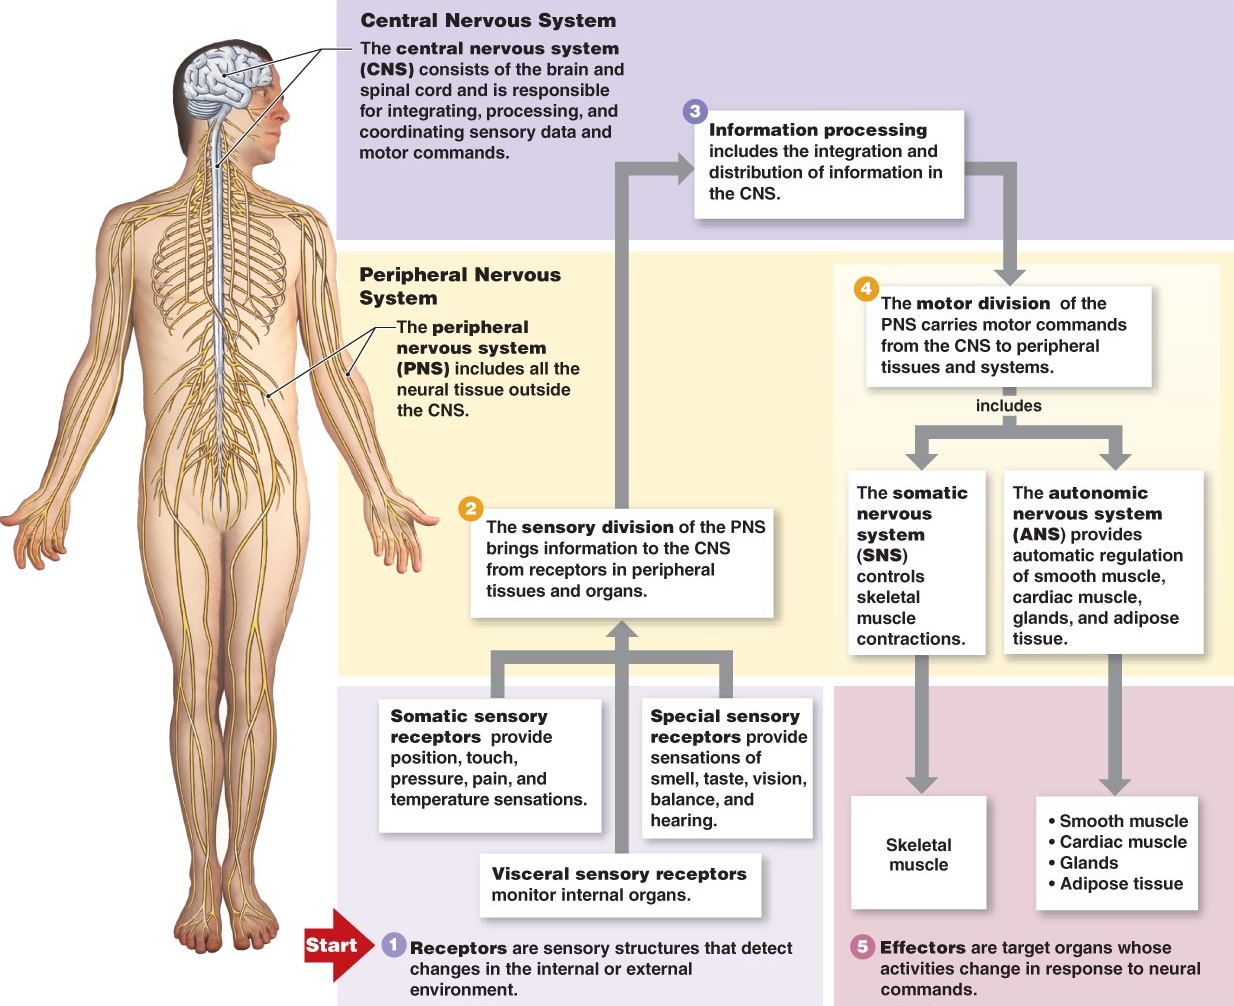
\includegraphics[scale=0.8]{figures/bProblemanalyse/Nervesys.jpg}
	\caption{Her ses et flowdiagram over, hvad der sker, når kroppen modtager et signal og skal processere dette om til en handling. Der ses desuden også en inddeling af CNS pg PNS med dets underdelinger. \cite{2015}}
	\label{Nersys}
\end{figure}

\section{Hjernens anatomi}
Cerebrum er encephalons største del og er involveret i sanseintegration, styring af frivillige bevægelser og højere intellektuelle funktioner, såsom tale og abstrakt tænkning. \cite{Academic2015b} Cerebrums ydre lag hedder cerebral cortex men kaldes hjernens grå substans. Her ligger nervers soma med dendritter. Cerebral cortex har forskellige centre, men kan også inddeles i højre og venstre halvdel. Delen af cerebral cortex der kontrollerer kroppens motorik med motor cortex kaldes gyrus præcentralis. Nerverne i dette område leder motoriske impulser til kroppens muskler igennem nervebanerne i den hvide substans, som indeholder nervernes axoner og fungerer derved som transportvej. \cite{Academic2015b,Martini2012,Stanfield2014} Disse axoner krydses i medulla oblongata og medulla spinalis og løber derefter til det modsatte legemeshalvdel fra, hvor impulsen afsendes. \cite{Martini2012}
